% This is samplepaper.tex, a sample chapter demonstrating the
% LLNCS macro package for Springer Computer Science proceedings;
% Version 2.20 of 2017/10/04
%
\documentclass[runningheads]{llncs}
%
%%%%%ДОБАВИЛ ДЛЯ РУССКОГО ТЕКСТА
\usepackage[utf8x]{inputenc}
\usepackage[english,russian]{babel}
\usepackage{cmap}
%%%%%
\usepackage{graphicx}

% Used for displaying a sample figure. If possible, figure files should
% be included in EPS format.
%
% If you use the hyperref package, please uncomment the following line
% to display URLs in blue roman font according to Springer's eBook style:
% \renewcommand\UrlFont{\color{blue}\rmfamily}

\begin{document}
%
\title{Comparison of dimensionality reduction schemes for parallel global optimization algorithms\thanks{Выполнено при поддержке РНФ -...}}
%
%\titlerunning{Abbreviated paper title}
% If the paper title is too long for the running head, you can set
% an abbreviated paper title here
%
\author{Konstantin Barkalov \and
Vladislav Sovrasov \and
Ilya Lebedev \and}
%
\authorrunning{F. Author et al.}
% First names are abbreviated in the running head.
% If there are more than two authors, 'et al.' is used.
%
\institute{
Lobachevsky State University of Nizhny Novgorod, Nizhny Novgorod, Russia
\email{konstantin.barkalov@itmm.unn.ru}\\
\email{sovrasov.vlad@gmail.com}\\
\email{ilya.lebedev@itmm.unn.ru}\\
\url{http://hpc-education.unn.ru/основные-напраления/глобальная-оптимизация} }
%
\maketitle              % typeset the header of the contribution
%
\begin{abstract}
This work considers a parallel algorithms for solving multi-extremal optimization problems. Algorithms are developed within the framework of the information-statistical approach and implemented in a parallel solver “Globalizer” . The optimization problem is solved by reducing the multidimensional problem to a set of joint one-dimensional problems that are solved in parallel. Five types of Peano-type space-filling curves are employed to reduce dimension. The results of computational experiments carried out on several hundred test problems are discussed. 

\keywords{Global optimization \and  Dimension reduction \and Parallel algorithms  \and Multidimensional multiextremal optimization  \and Global search algorithms  \and Parallel computations }
\end{abstract}
%
%
%

\section{Introduction}\label{sec:intro}

Global (or multiextremal) optimization problems are among the most complex problems
in both theory and practice of optimal decision making. In these kinds of problems,
the optimization criterion can have several local optima within the search domain.
The existence of several local optima makes
finding the global optimum difficult essentially, since it requires examining the whole feasible
search domain. The volume of computations for solving global optimization problems
can increase exponentially with increasing number of varied parameters.
\par
These global optimization problem features impose special requirements on the quality
of the optimization methods and on the software to implement these ones. The global
optimization methods should be highly efficient, and the software systems should be developed on
a good professional basis. In general, the global optimization problems can be solved at
a reasonable time by employing parallel computations on modern supercomputing systems only.
\par
The general state of the art in the field of global optimization is presented in a
number of key monographs  \cite{floudasPardGO}, \cite{horstTuyGO}, \cite{locatelliSchoenGO}, \cite{pinterGO}, \cite{strSergGO}, \cite{zilinskTornGO}, \cite{zhigljavskyRandGO}.
The development of optimization methods, which use the high-performance computational
systems to solve the time-consuming global optimization problems, is an area of
intensive research --- see, for instance, \cite{censorZeniosParGO}, \cite{ciegisHentyParGO},
\cite{luqueAlbaGA}, \cite{stronginGergelBarkalovParGO}, \cite{strSergGO}. The obtained
theoretical results provide the efficient solutions of many applied global
optimization problems in various fields of scientific and technical applications \cite{Famularo1999}, \cite{fasanoPinter2013},
\cite{floudasPardalosGOState}, \cite{Kvasov2015}, \cite{Menniti}, \cite{locatelliSchoenGO},
\cite{luqueAlbaGA}, \cite{pardalosZhigljavskyZilinskas2016}, \cite{pinterGO}.
\par
At the same time, the practical implementation of these global optimization algorithms
within the framework of industrial software systems is quite limited. In many cases,
software implementations are experimental in nature and are used by the developers
themselves to obtain the results from the computational experiments required for the
scientific publications. This situation originates from high development costs of the
professional software systems, which can be used by numerous users. In addition, the global
optimization problems could be solved in an automatic mode rarely because of the
complexity of these ones. The user should actively control the global search
process that implies an adequate level of qualification in the field of optimization
(particularly, the user should know and understand the global optimization methods well).
\par
In this work, the authors consider an approach to minimizing multiextremal functions  developed in ...????????
This allows problems to be solved in which function values may not be deter-mined for the entire search domain. Under this approach, solving multidimen-sional problems is reduced (using Peano-type space-filling curves) to solving equivalent one-dimensional problems.
It should be noted that standard approaches to algorithm parallelization are not quite applicable to global optimization. For example, the rules for selecting an-other iteration point are quite simple and do not require parallelization (as over-heads associated with organizing parallel computations will nullify any possible acceleration). Some acceleration can be achieved by parallelizing the computa-tion of function values describing the object to be optimized; however, this ap-proach is specific to each individual problem being solved.
The following approach looks more promising. The algorithm can be modified to run several trials in parallel. This approach provides the efficiency (as paral-lelization is applied to the most computation-intensive part of the problem solv-ing process) and generality (in that it applies to a wide range of global optimiza-tion algorithms). The approach, described in  \cite{Two_Level_Parallel} for unconstrained optimization, was used in this work for parallelizing constrained optimization algorithms.

\section{Statement of Multidimensional Global Optimization Problem}
In this paper, the core class of optimization problems, which can be solved using
Globalizer, is formulated. This class involves the multidimensional global
optimization problems without constraints, which can be defined in the following way:
\begin{equation}
\label{eq:task}
\begin{array}{cr}\\
  \varphi(y^*)=\min\{\varphi(y):y\in D\}, \\
  D=\{y\in \mathbf{R}^N:a_i\leq y_i\leq{b_i}, 1\leq{i}\leq{N}\}
\end{array}
\end{equation}
with the given boundary vectors  $a$ and  $b$. It is supposed, that the objective function \(\varphi(y)\) satisfies the Lipschitz condition
\begin{equation}
\label{eq:lip}
|\varphi(y_1)-\varphi(y_2)|\leq L\Vert y_1-y_2\Vert,y_1,y_2\in D,
\end{equation}
where \(L>0\) is the Lipschitz constant, and \(||\cdot||\) denotes the norm in \(\mathbf{R}^N\) space.
\par
Usually, the minimized function \(\varphi(y)\) is defined as a computational procedure,
according to which the value \(\varphi(y)\) can be calculated for any vector \(y\in D\)
(let us further call such a calculation \textit{a trial}). It is supposed that this procedure
is a time-consuming one. As a result, the overall time of solving the optimization
problem (\ref{eq:task}) is determined, first of all by the number of executed trials.
It should also be noted that the requirement of the Lipschitz condition (\ref{eq:lip})
is highly important, since an estimate of the global minimum can be constructed on the
basis of a finite number of computed values of the optimized function only in this case .
\par
As it has been shown earlier by many researchers
(see, for instance, \cite{floudasPardalosGOState}, \cite{horstTuyGO}, \cite{pinterGO}, \cite{strSergGO}),
finding the numerical estimate of the global optimum implies constructing a coverage of
the search domain \(D\). As a result, the computational costs of solving the global
optimization problems are readily very high even for a small number of varied parameters
(the dimensionality of the problem). A notable reduction in the volume of computations
can be achieved when the coverage of the search domain is non-uniform, i. e. the series
of trial points is only dense in a vicinity of the global optimum point. The construction
of such a non-uniform coverage could be provided in an adaptive way, when the selection
of the next trial points is determined by using the search information (the preceding
trial points and the values of the minimized function at these points) obtained in the course
of computations. This necessary condition complicates considerably the computational schemes
of global optimization methods since it implies a complex analysis of a large amount
of multidimensional search information. As a result, many optimization algorithms use
various approaches to the dimensional reduction \cite{pinterGO}, \cite{sergeyevStronginLera2013}, \cite{strongin1978}, \cite{stronginGergelBarkalovParGO}, \cite{strSergGO}.

\section{Methods of Dimension Reduction}
\subsection{Базовый алгоритм}

Within the framework of the information-statistical global optimization theory,
the Peano space-filling curves (or evolvents) \(y(x)\) mapping the interval \([0,1]\)
onto an \(N\)-dimensional hypercube \(D\) unambiguously are used for the dimensionality
reduction \cite{sergeyevStronginLera2013}, \cite{strongin1978}, \cite{stronginGergelBarkalovParGO}, \cite{strSergGO}.
\par
As a result of the reduction, the initial multidimensional global optimization
problem (\ref{eq:task}) is reduced to the following one-dimensional problem:
\begin{equation}
\label{eq:oneDimTask}
\varphi(y(x^*))=\min\{\varphi(y(x)):x\in [0,1]\}.
\end{equation}
\par
It is important to note that this dimensionality reduction scheme transforms the minimized
Lipschitzian function from (\ref{eq:task}) to the corresponding one-dimensional
function \(\varphi(y(x))\), which satisfies the uniform H{\"o}lder condition, i. e.
\begin{equation}
\label{eq:holder}
|\varphi(y(x_1))-\varphi(y(x_2))|\leq H{|x_1-x_2|}^{\frac{1}{N}}, x_1,x_2\in[0,1],
\end{equation}
where the constant $H$ is defined by the relation \(H=2L\sqrt{N+3}\), \(L\) is the Lipschitz
constant from (\ref{eq:lip}), and \(N\) is the dimensionality of the optimization problem (\ref{eq:task}).
\par
The algorithms for the numerical construction of the Peano curve approximations are
given in \cite{strSergGO}. As an illustration, an approximation of the Peano curve
for the third density level is shown in Figure \ref{fig:peanoC}. Figure \ref{fig:peanoC}
demonstrates the movement order in a two-dimensional domain to construct the Peano
curve approximation; the precision of the Peano curve approximation is determined by the
density level used in the construction.
\begin{figure}
    \centering
    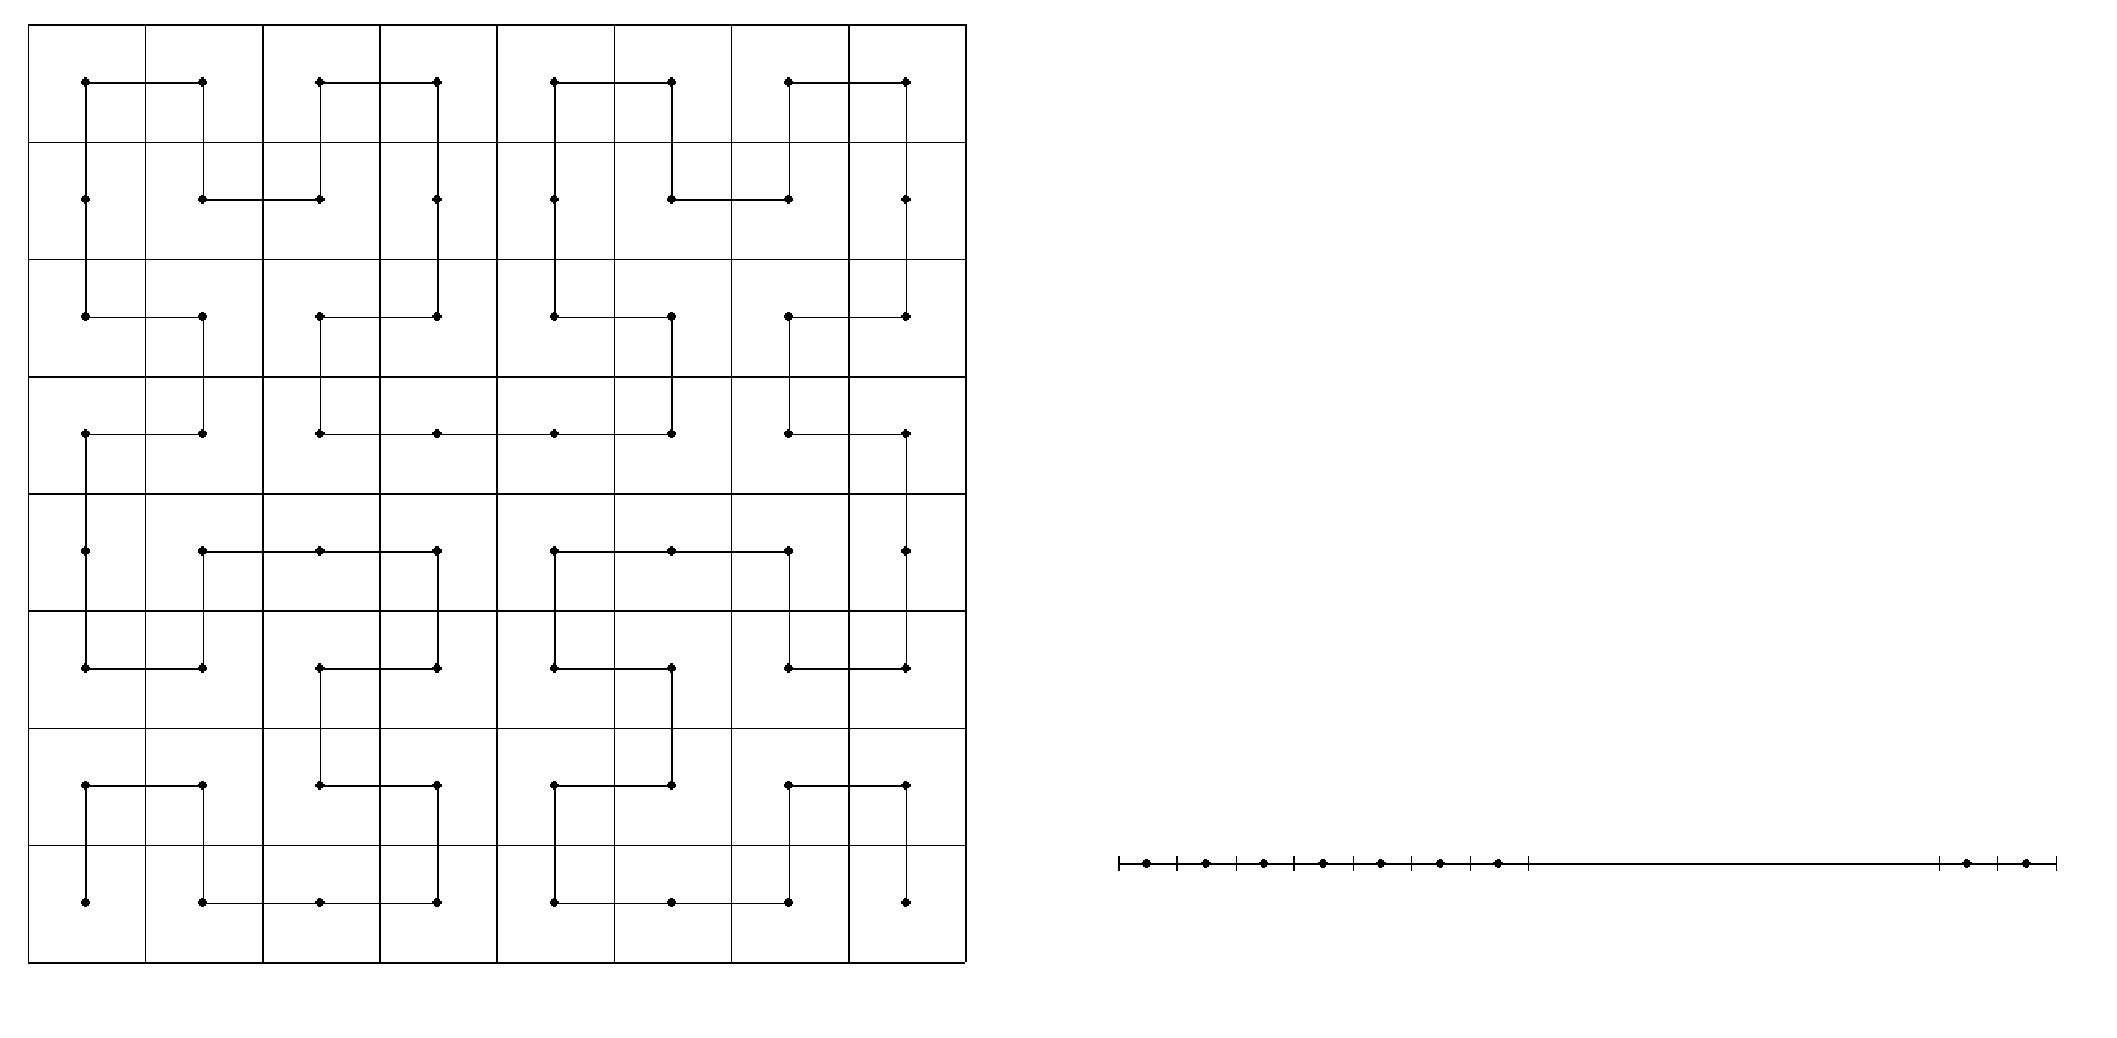
\includegraphics[width=0.85\textwidth]{pictures/peanoC.eps}
    \caption{A Peano curve approximation for the third density level}
    \label{fig:peanoC}
\end{figure}

\par
The computational scheme obtained as a result of the dimensionality reduction consists of the following
(see Figure \ref{fig:peanoCUsage}):
\begin{itemize}
  \item The optimization algorithm performs the minimization of the reduced one-dimensional
  function \(\varphi(y(x))\) from (\ref{eq:oneDimTask}),
  \item After determining the next trial point \(x\), a multidimensional image \(y\) is calculated by using the
mapping \(y(x)\),
  \item The value of the initial multidimensional function \(\varphi(y)\) is calculated at the point \(y\in D\),
  \item The calculated value \(z=\varphi(y)\) is used further as the value of the reduced one-dimensional function \(\varphi(y(x))\) at the point \(x\).
\end{itemize}

\begin{figure}
    \centering
    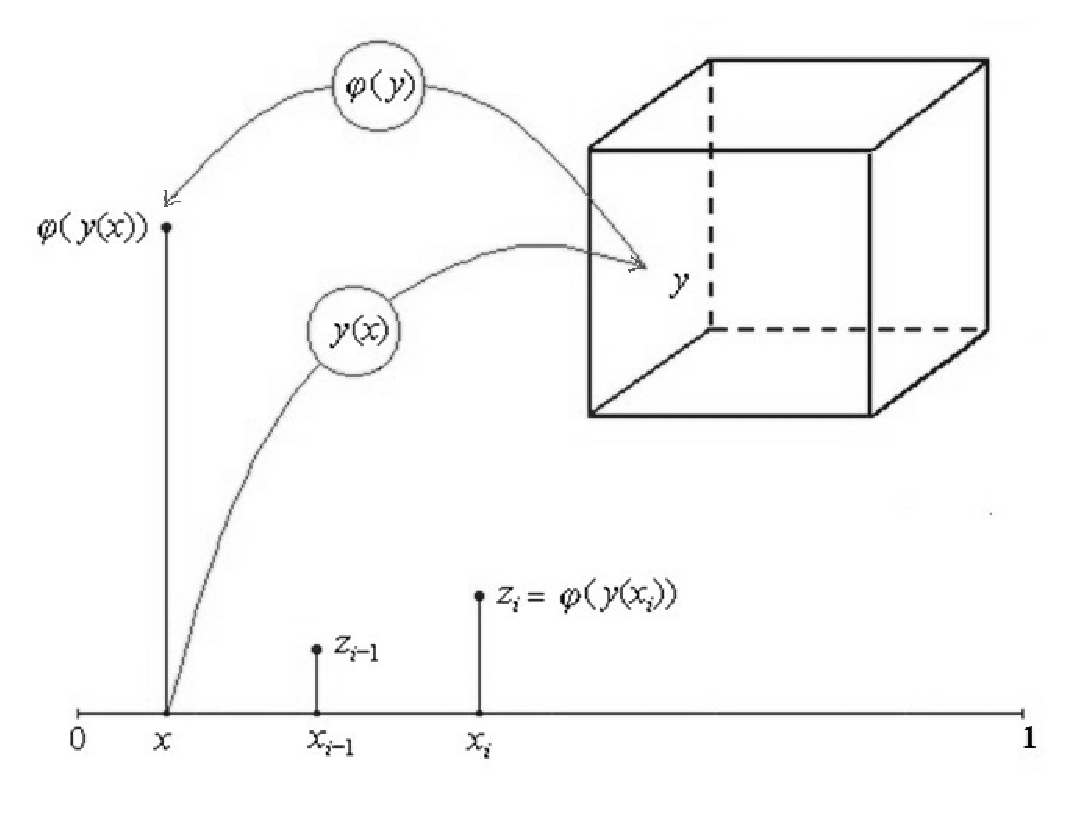
\includegraphics[width=0.55\textwidth]{pictures/peanoCUsage.eps}
    \caption{The computational scheme for obtaining the value of the reduced one-dimensional function \(\varphi(y(x))\)}
    \label{fig:peanoCUsage}
\end{figure}

\subsection{Сдвиговые}
s
\subsection{Вращаемые}
s
\subsection{Еще одни развертки}
s
\subsection{Гладкие}
s
\section{Parallel Computations for Solving Global Optimization Problems.}
\subsection{Core Multidimensional Algorithm of Global Search}

The information-statistical theory of global optimization formulated in \cite{strongin1978}, \cite{strSergGO} has
served as a basis for the development of a large number of efficient multiextremal optimization
methods \cite{barkalovGergel2014}, \cite{gergel1996}, \cite{gergel1997}, \cite{grishaginStrongin1984}, \cite{Pizzuti}, \cite{sergeyev1995}, \cite{sergeyev1999}, \cite{sergeyevGrishagin2001}, \cite{sergeyevStronginLera2013}, \cite{Famularo2001}.
\par
The optimization methods applied in Globalizer are based on the MAGS method, which can be presented as follows --- see \cite{strongin1978}, \cite{strSergGO}.
\par
Let us introduce a simpler notation for the optimization problem being solved
\begin{equation}
\label{eq:oneDimFunc}
f(x) = \varphi(y(x)):x\in [0,1].
\end{equation}
\par
The initial iteration of the algorithm is performed at an arbitrary point \mbox{\(x^1\in(0,1)\)}.
Then, let us suppose that \(k\), \(k\ge 1\), optimization iterations have been completed already.
The selection of the trial point \(x^{k+1}\) for the next iteration is performed according to the following rules.
\par
\textit{Rule 1}. Renumber the points of the preceding trials by the lower indices in order of increasing value of coordinates
\begin{equation}
  \label{step1}
0=x_0<x_1<...<x_{k+1}=1,
\end{equation}
the points \(x_0\), \(x_{k+1}\) were introduced additionally for the convenience of further
explanation, the values of the minimized function \(z_0\), \(z_{k+1}\) at these points are undefined.
\par
\textit{Rule 2}. Compute the current estimate of the H{\"o}lder constant \(H\) from (\ref{eq:holder})
\begin{equation} \label{step2}
M=\max_{1 < i\leq k}\frac{|z_i-z_{i-1}|}{\rho_i}, \;
m = \left\{
   \begin{array}{lr}
     rM, & M > 0,\\
     1, & M = 0,
   \end{array}
  \right.
\end{equation}
as the maximum of the relative differences of the minimized function values on the
set of previously executed trial points \(x_i,1\leq i\leq k\) from (\ref{step1}).
Hereafter, \(\rho_i=(x_i-x_{i-1})^\frac{1}{N},1\leq i\leq k+1\). The
constant \(r\), \(r>1\), is the reliability parameter of the algorithm.
\par
\textit{Rule 3}. Compute the characteristics \(R(i)\) for each interval \((x_{i-1},x_i),1\leq i\leq k+1\), where
\[
R(i)=2\rho_i-4\frac{z_i}{m},\quad i=1,
\]
\begin{equation} \label{step3}
R(i)=\rho_i+\frac{(z_i-z_{i-1})^2}{m^2\rho_i}-2\frac{z_i+z_{i-1}}{m},\quad 1<i<k+1, \\
\end{equation}
\[
R(i)=2\rho_{i}-4\frac{z_{i-1}}{m},\quad i=k+1.
\]

\par
\textit{Rule 4}. Determine the interval with the maximum characteristic
\begin{equation} \label{step4}
R(t)=\max_{1\leq i \leq k+1}R(i).
\end{equation}
\par
\textit{Rule 5}. Execute a new trial at the point \(x^{k+1}\) located within the interval
with the maximum characteristic from (\ref{step4})
\begin{equation} \label{step5}
  x^{k+1}=\frac{x_t+x_{t-1}}{2}-\mathrm{sign}(z_{t}-z_{t-1})\frac{1}{2r}\left[\frac{r|z_{t}-z_{t-1}|}{m}\right]^N,\; \textrm{ if } 1<t<k+1,
\end{equation}
\[
  x^{k+1}=\frac{x_t+x_{t-1}}{2},\; \textrm{ if } t=1 \textrm{ or } t=k+1.
\]

\par
The stopping condition, which terminated the trials, is defined by the inequality
\begin{equation}
  \label{eq:stop_1}
\rho_t<\varepsilon
\end{equation}
for the interval with the maximum characteristic from (\ref{step4}) and \(\varepsilon >0\) is the predefined
accuracy of the optimization problem solution. If the stopping condition is not satisfied,
the index \(k\) is incremented by 1, and the new global optimization iteration is executed.
\par
In order to explain the algorithm presented above, let us note the following.
The characteristics \(R(i), 1\leq i\leq k+1\), calculated according to (\ref{step3}) could
be interpreted as some measures of importance of the intervals with respect to the
expected location of the global minimum point. Thus, the rules (\ref{step4}) and (\ref{step5}) for selecting
the interval of the next trial become more clear --- the point of every next
global optimization iteration is selected within the interval, where the global minimum
point can be found most likely.
\par
The convergence conditions of the described algorithm are given, for example, in \cite{strSergGO}.

\subsection{Параллельные множественные отображения}

The reduction of the multidimensional problems to the one-dimensional ones using evolvents has such important properties as the continuity and preservation of boundedness of function divided differences. However, a partial loss of in-formation on the nearness of the points in the multidimensional space takes place since a point \mbox{\(x\in[0,1]\)} has only the left and the right neighbors while the corresponding point  \mbox{\(y(x)\in R^N\)} has the neighbors in \(2N\) directions. As a result, when using the mappings like Peano curve the images \(y',y''\), which are close to each other in the N-dimensional space can correspond to the preimages \(x',x''\), which can be far away from each other in the interval [0,1]. This property results in the excess computations since several limit points \(x',x''\) of the trial sequence generated by the index method in the interval [0,1] can correspond to a single limit point y in the \(N\)-dimensional space.
\par
One of the possible ways to overcome this disadvantage consists in using the multiple mapping \(Y^S (x)={y^1 (x),…,y^S (x)}\) instead of single evolvent \(y(x)\). To construct the set \(Y^S (x)\) different approaches can be used. For example, in \cite{strSergGO} a scheme was implemented, according to which each evolvent \(y^i (x)\) from \(Y^S (x)\) is constructed as a result of shifting the original evolvent \(y^0 (x)\) along the main diagonal of the hypercube \(D\). The set of Peano curves thus constructed allows one to obtain \(y',y''\) from \(D\) for any close multidimensional images, which differ only in one coordinate, close preimages \(x',x''\) from the interval [0,1] for the evolvent \(y^s (x),1≤s≤S\).
Using the multiple mapping allows solving initial problem (1) by parallel solving the problems
\par

\[
\min\{\varphi(y^s(x)):x\in [0,1]\}, 1≤s≤S
\]

on a set of intervals [0,1] by the index method. Each one-dimensional problem is solved on a separate processor. The trial results at the point \(x^k\) obtained for the problem being solved by particular processor are interpreted as the results of the trials in the rest problems (in the corresponding points \(x^(k_1 ),…,x^(k_S ))\). In this approach, a trial at the point \(x^k \in [0,1]\) executed in the framework of the \(s\)-th problem, consists in the following sequence of operations.
\par
1. Determine the image \(y^k=y^s (x^k)\) for the evolvent \(y^s (x)\).
\par
2. Inform the rest of processors about the start of the trial execution at the point\( y^k\) (the blocking of the point \(y^k\) ).
\par
3. Determine the preimages \(x{}^{k_s}  \in [0,1], 1≤s≤S\), of the point \(y^k\) and interpret the trial executed at the point \(y^k \in D \) as the execution of the trials in the \(S\) points \(x{}^{k_1} ,…,x{}^{k_s} \) 
\par
4. Inform the rest of processors about the trial results at the point \(y^k\).
\par

The decision rules for the proposed parallel algorithm, in general, are the same as the rules of the sequential algorithm (except the method of the trial execution). Each processor has its own copy of the software realizing the computations of the problem functions and the decision rule of the index algorithm. For the organization of the interactions among the processors, the queues are created on each processor, where the processors store the information on the executed iterations in the form of the tuples: the processor number \(s\), the trial point \(x{}^{k_s}\).
\par
The proposed parallelization scheme was implemented with the use of MPI technology. Main features of implementation consist in the following. A separate MPI-process is created for each of \(S\) one-dimensional problems being solved, usually, one process per one processor employed. Each process can use p threads, usually one thread per an accessible core.
\par
At every iteration of the method, the process with the index \(s,0≤ s< S\) performs p trials in parallel at the points \(x^(s+iS),0≤i<p\). At that, each process stores all \(S_p\) points, and an attribute indicating whether this point is blocked by another process or not is stored for each point. Let us remind that the point is blocked if the process starts the execution of a trial at this point.
\par
At every iteration of the algorithm, operating within the \(s\)-th process, determines the coordinates of p «its own» trial points. Then, the interchange of the coordinates of images of the trial points \(y^(s+iS),0≤i<p, 0≤ s< S\) is performed (from each process to each one). After that, the preimages \(x^(q+iS),0≤ q<S,q≠s\) of the points received by the \(s\)-th process from the neighbor ones are determined with the use of the evolvent \(y^s (x)\). The points blocked within the \(s\)-th process will correspond to the preimages obtained. Then, each process performs the trials at the non-blocked points, the computations are performed in parallel using OpenMP. The results of the executed trials (the index of the point, the computed values of the problem functions, and the attribute of unblocking of this point) are transferred to all rest processes. All the points are added to the search information database, and the transition to the next iteration is performed.
\par

\section{Results of Numerical Experiments}
s
\subsection{Сравнение последовательных сдвиговых и вращаемых разверток}
s
\subsection{Параллельные вращаемые развертки}
s
\subsection{Параллельные вращаемые развертки для задач большой размерности}
s
\section{Вывод о целесообразности применения того или иного вида разверток для того или иного вида задач}
s

\section{First Section}
\subsection{A Subsection Sample}
Please note that the first paragraph of a section or subsection is
not indented. The first paragraph that follows a table, figure,
equation etc. does not need an indent, either.

Subsequent paragraphs, however, are indented.

\subsubsection{Sample Heading (Third Level)} Only two levels of
headings should be numbered. Lower level headings remain unnumbered;
they are formatted as run-in headings.

\paragraph{Sample Heading (Fourth Level)}
The contribution should contain no more than four levels of
headings. Table~\ref{tab1} gives a summary of all heading levels.

\begin{table}
\caption{Table captions should be placed above the
tables.}\label{tab1}
\begin{tabular}{|l|l|l|}
\hline
Heading level &  Example & Font size and style\\
\hline
Title (centered) &  {\Large\bfseries Lecture Notes} & 14 point, bold\\
1st-level heading &  {\large\bfseries 1 Introduction} & 12 point, bold\\
2nd-level heading & {\bfseries 2.1 Printing Area} & 10 point, bold\\
3rd-level heading & {\bfseries Run-in Heading in Bold.} Text follows & 10 point, bold\\
4th-level heading & {\itshape Lowest Level Heading.} Text follows & 10 point, italic\\
\hline
\end{tabular}
\end{table}


\noindent Displayed equations are centered and set on a separate
line.
\begin{equation}
x + y = z
\end{equation}
Please try to avoid rasterized images for line-art diagrams and
schemas. Whenever possible, use vector graphics instead (see
Fig.~\ref{fig1}).

\begin{figure}
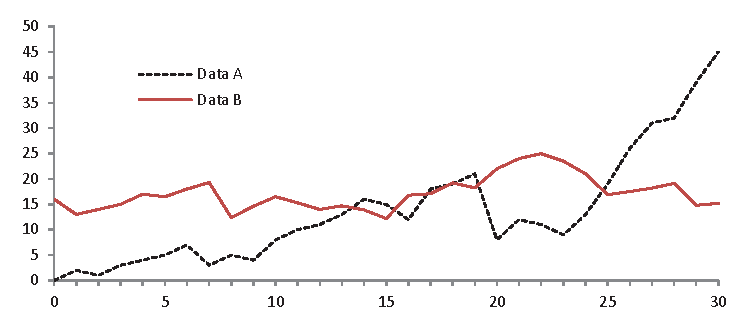
\includegraphics[width=\textwidth]{fig1.eps}
\caption{A figure caption is always placed below the illustration.
Please note that short captions are centered, while long ones are
justified by the macro package automatically.} \label{fig1}
\end{figure}

\begin{theorem}
This is a sample theorem. The run-in heading is set in bold, while
the following text appears in italics. Definitions, lemmas,
propositions, and corollaries are styled the same way.
\end{theorem}
%
% the environments 'definition', 'lemma', 'proposition', 'corollary',
% 'remark', and 'example' are defined in the LLNCS documentclass as well.
%
\begin{proof}
Proofs, examples, and remarks have the initial word in italics,
while the following text appears in normal font.
\end{proof}
For citations of references, we prefer the use of square brackets
and consecutive numbers. Citations using labels or the author/year
convention are also acceptable. The following bibliography provides
a sample reference list with entries for journal
articles~\cite{ref_article1}, an LNCS chapter~\cite{ref_lncs1}, a
book~\cite{ref_book1}, proceedings without editors~\cite{ref_proc1},
and a homepage~\cite{ref_url1}. Multiple citations are grouped
\cite{ref_article1,ref_lncs1,ref_book1},
\cite{ref_article1,ref_book1,ref_proc1,ref_url1}.
%
% ---- Bibliography ----
%
% BibTeX users should specify bibliography style 'splncs04'.
% References will then be sorted and formatted in the correct style.
%
% \bibliographystyle{splncs04}
% \bibliography{mybibliography}
%
\begin{thebibliography}{107}


\bibitem{barkalovGergel2014}
\newblock K. Barkalov and V. Gergel,
\newblock \emph{\emph{Multilevel scheme of dimensionality reduction for parallel global search algorithms}},
\newblock in \emph{Proceedings of the 1st International Conference on Engineering and Applied Sciences Optimization}, (2014), 2111--2124.

\bibitem{barkalovGergel2015}% (MR3539505) [10.1007/s10898-016-0411-y]
\newblock K. Barkalov and V. Gergel,
\newblock \emph{\emph{Parallel global optimization on GPU}},
\newblock \emph{J. Glob. Optim.}, \textbf{66} (2016), 3--20.

\bibitem{barkalovGergelLebedev2015} %[10.1007/978-3-319-21909-7_31]
\newblock K. Barkalov, V. Gergel and I. Lebedev,
\newblock \emph{\emph{Use of Xeon Phi coprocessor for solving global optimization problems}},
\newblock \emph{LNCS}, \textbf{9251} (2015), 307--318.

\bibitem{barkalovGergelLebedevSysoev2015}
\newblock K. Barkalov, V. Gergel, I. Lebedev and A. Sysoev,
\newblock \emph{\emph{Solving the global optimization problems on heterogeneous cluster systems}},
\newblock in \emph{CEUR Workshop Proceedings}, \textbf{1482} (2015), 411--419.

\bibitem{Barkalov2013}% [10.1007/978-3-642-39958-9_14]
\newblock K. Barkalov, A. Polovinkin, I. Meyerov, S. Sidorov and N. Zolotykh,
\newblock \emph{\emph{SVM regression parameters optimization using parallel global search algorithm}},
\newblock \emph{LNCS}, \textbf{7979} (2013), 154--166.

\bibitem{bussieckMeeraus2004} (MR3618583)% [10.1007/978-1-4613-0215-5_8]
\newblock M. R. Bussieck and A. Meeraus,
\newblock \emph{\emph{General algebraic modeling system (GAMS)}},
\newblock in \emph{Modeling Languages in Mathematical Optimization} (ed. J. Kallrath), Springer, (2004), 137--157.

\bibitem{censorZeniosParGO}% (MR1486040)
\newblock Y. Censor and S. A. Zenios,
\newblock \emph{Parallel Optimization: Theory, Algorithms, and Applications},
\newblock Oxford University Press, 1998.

\bibitem{ciegisHentyParGO} (MR2499546)% [10.1007/978-0-387-09707-7]
\newblock R. \v Ciegis, D. Henty, B. K\aa gstr\"om and J. \v Zilinskas,
\newblock \emph{Parallel Scientific Computing and Optimization: Advances and Applications},
\newblock Springer, 2009.

\bibitem{iosoDescription}
\newblock I. N. Egorov, G. V. Kretinin, I. A. Leshchenko and S. V. Kuptzov,
\newblock \emph{\emph{IOSO optimization toolkit --- novel software to create better design}},
\newblock in \emph{9th AIAA/ISSMO Symposium on Multidisciplinary Analysis and Optimization}, 2002. Available from \url{http://www.iosotech.com/text/2002\_4329.pdf}.

\bibitem{Famularo1999} %(MR1827451) [10.1016/S0005-1098(99)00058-8]
\newblock D. Famularo, P. Pugliese and Y. D. Sergeyev,
\newblock \emph{\emph{A global optimization technique for checking parametric robustness}},
\newblock \emph{Automatica}, \textbf{35} (1999), 1605--1611.

\bibitem{fasanoPinter2013}% (MR3013800) [10.1007/978-1-4614-4469-5]
\newblock G. Fasano and J. D. Pint\'er,
\newblock \emph{Modeling and Optimization in Space Engineering},
\newblock Springer, 2013.

\bibitem{floudasPardalosGOState} %(MR1390521) [10.1007/978-1-4613-3437-8]
\newblock C. A. Floudas and M. P. Pardalos,
\newblock \emph{State of the Art in Global Optimization: Computational Methods and Applications},
\newblock Kluwer Academic Publishers, Dordrecht, 1996.

\bibitem{floudasPardGO}% (MR1147432) [10.1007/s10898-008-9332-8]
\newblock C. A. Floudas and M. P. Pardalos,
\newblock \emph{Recent Advances in Global Optimization},
\newblock Princeton University Press, 2016.

\bibitem{Gablonsky} %(MR1856800) [10.1023/A:1017930332101]
\newblock J. M. Gablonsky and C. T. Kelley,
\newblock \emph{\emph{A locally-biased form of the DIRECT algorithm}},
\newblock \emph{J. Glob. Optim.}, \textbf{21} (2001), 27--37.

\bibitem{gavianoKvasovLeraSergeev2003} %(MR2077342) [10.1145/962437.962444]
\newblock M. Gaviano, D. E. Kvasov, D. Lera and Y. D. Sergeev,
\newblock \emph{\emph{Software for generation of classes of test functions with known local and global minima for global optimization}},
\newblock \emph{ACM Trans. Math. Software}, \textbf{29} (2003), 469--480.

\bibitem{gergelLebedev2015}% [10.1016/j.procs.2015.11.008]
\newblock V. Gergel and I. Lebedev,
\newblock \emph{\emph{Heterogeneous parallel computations for solving global optimization problems}},
\newblock \emph{Procedia Comput. Sci.}, \textbf{66} (2015), 53--62.

\bibitem{gergel1993}
\newblock V. Gergel,
\newblock \emph{\emph{A software system for multi-extremal optimization}},
\newblock \emph{Eur. J. Oper. Res.}, \textbf{65} (1993), 305--313.

\bibitem{gergel1996}% (MR1399766)
\newblock V. Gergel,
\newblock \emph{\emph{A method for using derivatives in the minimization of multiextremum functions}},
\newblock \emph{Comput. Math. Math. Phys.}, \textbf{36} (1996), 729--742.

\bibitem{gergel1997} %(MR1443089) [10.1023/A:1008290629896]
\newblock V. Gergel,
\newblock \emph{\emph{A global optimization algorithm for multivariate functions with Lipschitzian first derivatives}},
\newblock \emph{J. Glob. Optim.}, \textbf{10} (1997), 257--281.

\bibitem{gergel2013} %[doi:10.1016/j.procs.2013.05.164]
\newblock V. Gergel, et al.,
\newblock \emph{\emph{High performance computing in biomedical applications}},
\newblock \emph{Procedia Computer Science}, \textbf{18} (2013), 10--19.

\bibitem{gergel2015}% [10.15866/ireaco.v8i1.4935]
\newblock V. Gergel, et al.,
\newblock \emph{\emph{Recognition of surface defects of cold-rolling sheets based on method of localities}},
\newblock \emph{International Review of Automatic Control, } \textbf{8} (2015), 51--55.

\bibitem{gergelSidorov2015}% [10.1007/978-3-319-21909-7_49]
\newblock V. Gergel and S. Sidorov,
\newblock \emph{\emph{A two-level parallel global search algorithm for solving computationally intensive multi-extremal optimization problems}},
\newblock \emph{LNCS}, \textbf{9251} (2015), 505--515.

\bibitem{grishaginStrongin1984}% (MR785497)
\newblock V. A. Grishagin and R. G. Strongin,
\newblock \emph{\emph{Optimization of multi-extremal functions subject to monotonically unimodal constraints}},
\newblock \emph{Engineering Cybernetics}, \textbf{5} (1984), 117--122.

\bibitem{holmstromEdvall2004}% [10.1007/978-1-4613-0215-5_19]
\newblock K. Holmstrm and M. M. Edvall,
\newblock \emph{\emph{The TOMLAB optimization environment}},
\newblock \emph{Modeling Languages in Mathematical Optimization}, Springer, (2004), 369--376.

\bibitem{horstTuyGO}% (MR1102239) [10.1007/978-3-662-03199-5]
\newblock R. Horst and H. Tuy,
\newblock \emph{Global Optimization: Deterministic Approaches},
\newblock Springer-Verlag, Berlin, 1990.

\bibitem{Jones} (MR1246501)% [10.1007/BF00941892]
\newblock D. R. Jones, C. D. Perttunen and B. E. Stuckman,
\newblock \emph{\emph{Lipschitzian optimization without the Lipschitz constant}},
\newblock \emph{J. Optim. Theory Appl.}, \textbf{79} (1993), 157--181.

\bibitem{kearfott2009}%(MR2554906) [10.1080/10556780802614051]
\newblock R. B. Kearfott,
\newblock \emph{\emph{GlobSol user guide}},
\newblock \emph{Optim. Methods Softw.}, \textbf{24} (2009), 687--708.

\bibitem{Kvasov2015}% (MR3585540) [10.1016/j.advengsoft.2014.09.014]
\newblock D. E. Kvasov and Y. D. Sergeyev,
\newblock \emph{\emph{Deterministic approaches for solving practical black-box global optimization problems}},
\newblock \emph{Adv. Eng. Softw.}, \textbf{80} (2015), 58--66.

\bibitem{Menniti}% [10.1016/j.epsr.2007.10.009]
\newblock D. E. Kvasov, D. Menniti, A. Pinnarelli, Y. D. Sergeyev and N. Sorrentino,
\newblock \emph{\emph{Tuning fuzzy power-system stabilizers in multi-machine systems by global optimization algorithms based on
 efficient domain partitions}},
\newblock \emph{Electric Power Systems Research}, \textbf{78} (2008), 1217--1229.

\bibitem{Pizzuti}% (MR1971214) [10.1007/s00211-002-0419-8]
\newblock D. E. Kvasov, C. Pizzuti and Y. D. Sergeyev,
\newblock \emph{\emph{Local tuning and partition strategies for diagonal GO methods}},
\newblock \emph{Numerische Mathematik}, \textbf{94} (2003), 93--106.

\bibitem{liberti2009}% (MR2206955) [10.1007/0-387-30528-9_8]
\newblock L. Liberti,
\newblock \emph{\emph{Writing global optimization software}},
\newblock in \emph{Nonconvex Optimization and Its Applications}, Springer, \textbf{84} (2006), 211--262.


\bibitem{linSchrage2009}% (MR2554904) [10.1080/10556780902753221]
\newblock Y. Lin and L. Schrage,
\newblock \emph{\emph{The global solver in the LINDO API}},
\newblock \emph{Optim. Methods Softw.}, \textbf{24} (2009), 657--668.

\bibitem{locatelliSchoenGO}% (MR3136805) [10.1137/1.9781611972672]
\newblock M. Locatelli and F. Schoen,
\newblock \emph{Global Optimization: Theory, Algorithms and Applications},
\newblock SIAM, 2013.

\bibitem{luqueAlbaGA}% (MR2808873) [10.1007/978-3-642-22084-5]
\newblock G. Luque and E. Alba,
\newblock \emph{Parallel Genetic Algorithms. Theory and Real World Applications},
\newblock Springer-Verlag, Berlin, 2011.

\bibitem{mongeauKarsentyRouze2000} %(MR1785196) [10.1080/10556780008805783]
\newblock M. Mongeau, H. Karsenty, V. Rouz$\acute{e}$ and J. B. Hiriart-Urruty,
\newblock \emph{\emph{Comparison of public-domain software for black box global optimization}},
\newblock \emph{Optim. Methods Softw.}, \textbf{13} (2000), 203--226.

\bibitem{mullen2014} %[10.18637/jss.v060.i06]
\newblock K. M. Mullen,
\newblock \emph{\emph{Continuous global optimization in R}},
\newblock \emph{J. Stat. Softw.}, \textbf{60} (2014).

\bibitem{pardalosZhigljavskyZilinskas2016}% (MR2361744) [10.1007/978-3-319-29975-4]
\newblock M. P. Pardalos, A. A. Zhigljavsky and J. \v Zilinskas,
\newblock \emph{Advances in Stochastic and Deterministic Global Optimization},
\newblock Springer, 2016.

\bibitem{pinterGO}% (MR1374104) [10.1007/978-1-4757-2502-5]
\newblock J. D. Pint\'er,
\newblock \emph{Global Optimization in Action (Continuous and Lipschitz Optimization: Algorithms, Implementations and Applications)},
\newblock Kluwer Academic Publishers, Dordrecht, 1996.

\bibitem{pinter2009}% (MR2528693)
\newblock J. D. Pint\'er,
\newblock \emph{\emph{Software development for global optimization}},
\newblock \emph{Lectures on Global Optimization. Fields Institute Communications}, \textbf{55} (2009), 183--204.

\bibitem{riosSahinidis2013} %(MR3070154) [10.1007/s10898-012-9951-y]
\newblock L. M. Rios and N. V. Sahinidis,
\newblock \emph{\emph{Derivative-free optimization: a review of algorithms and comparison of software implementations}},
\newblock \emph{J. Glob. Optim.}, \textbf{56} (2013), 1247--1293.

\bibitem{sahinidis1996} %(MR1376505) [10.1007/BF00138693]
\newblock N. V. Sahinidis,
\newblock \emph{\emph{BARON: A general purpose global optimization software package}},
\newblock \emph{J. Glob. Optim.}, \textbf{8} (1996), 201--205.

\bibitem{sergeyev1995} %(MR1358808) [10.1137/0805041]
\newblock Y. D. Sergeyev,
\newblock \emph{\emph{An information global optimization algorithm with local tuning}},
\newblock \emph{SIAM J. Optim.}, \textbf{5} (1995), 858--870.

\bibitem{sergeyev1999}% (MR1699326)
\newblock Y. D. Sergeyev,
\newblock \emph{\emph{Multidimensional global optimization using the first derivatives}},
\newblock \emph{Comput. Math. Math. Phys.}, \textbf{39} (1999), 743--752.

\bibitem{sergeyevKvasov2006}% (MR2197562) [10.1137/040621132]
\newblock Y. D. Sergeyev and D. E. Kvasov,
\newblock \emph{\emph{Global search based on efficient diagonal partitions and a set of Lipschitz constants}},
\newblock \emph{SIAM Journal on Optimization}, \textbf{16} (2006), 910--937.

\bibitem{sergeyevGrishagin2001}% (MR1825071) [10.1023/A:1010185125012]
\newblock Y. D. Sergeyev and V. A. Grishagin,
\newblock \emph{\emph{Parallel asynchronous global search and the nested optimization scheme}},
\newblock \emph{J. Comput. Anal. Appl.}, \textbf{3} (2001), 123--145.

\bibitem{sergeyevStronginLera2013}% (MR3113120) [10.1007/978-1-4614-8042-6]
\newblock Y. D. Sergeyev, R. G. Strongin and D. Lera,
\newblock \emph{Introduction to Global Optimization Exploiting Space-filling Curves},
\newblock Springer, 2013.

\bibitem{Famularo2001}% (MR1866703) [10.1023/A:1012391611462]
\newblock Y. D. Sergeyev, D. Famularo and P. Pugliese,
\newblock \emph{\emph{Index branch-and-bound algorithm for Lipschitz univariate global optimization with multiextremal constraints}},
\newblock \emph{J. Glob. Optim.}, \textbf{21} (2001), 317--341.

\bibitem{strongin1978}% (MR509033)
\newblock R. G. Strongin,
\newblock \emph{Numerical Methods in Multi-Extremal Problems (Information-Statistical Algorithms)},
\newblock Moscow: Nauka, In Russian, 1978.

\bibitem{strongin1992}% (MR1263606) [10.1007/BF00122428]
\newblock R. G. Strongin,
\newblock \emph{\emph{Algorithms for multi-extremal mathematical programming problems employing a set of joint space-filling curves}},
\newblock \emph{J. Glob. Optim.}, \textbf{2} (1992), 357--378.

\bibitem{stronginGergelBarkalovParGO}
\newblock R. G. Strongin, V. P. Gergel, V. A. Grishagin and K. A. Barkalov,
\newblock \emph{Parallel Computations for Global Optimization Problems},
\newblock Moscow State University (In Russian), Moscow, 2013.

\bibitem{strSergGO}5 (MR1797058) [10.1007/978-1-4615-4677-1]
\newblock R. G. Strongin and Y. D. Sergeyev,
\newblock \emph{Global Optimization with Non-convex Constraints. Sequential and Parallel Algorithms},
\newblock Kluwer Academic Publishers, Dordrecht (2000, 2nd ed. 2013, 3rd ed. 2014).

\bibitem{zilinskTornGO}% (MR1100586) [10.1007/3-540-50871-6]
\newblock A. T\"orn and A. \v Zilinskas,
\newblock \emph{Global Optimization},
\newblock Springer, 1989.

\bibitem{venkataraman2009}
\newblock P. Venkataraman,
\newblock \emph{Applied Optimization with MATLAB Programming},
\newblock John Wiley \& Sons, 2009.

\bibitem{zhigljavskyRandGO}% (MR1187048) [10.1007/978-94-011-3436-1]
\newblock A. A. Zhigljavsky,
\newblock \emph{Theory of Global Random Search},
\newblock Kluwer Academic Publishers, Dordrecht, 1991.

\bibitem{Two_Level_Parallel}
Gergel, V., Sidorov, S.: A Two-Level Parallel Global Search Algorithm for Solution of Computationally Intensive Multiextremal Optimization Problems. In: Malyshkin, V. (Ed.) PaCT 2015, LNCS, vol. 9251, pp. 505-515. Springer, Heidelberg (2015)

\bibitem{ref_article1}
Author, F.: Article title. Journal \textbf{2}(5), 99--110 (2016)

\bibitem{ref_lncs1}
Author, F., Author, S.: Title of a proceedings paper. In: Editor,
F., Editor, S. (eds.) CONFERENCE 2016, LNCS, vol. 9999, pp. 1--13.
Springer, Heidelberg (2016). \doi{10.10007/1234567890}

\bibitem{ref_book1}
Author, F., Author, S., Author, T.: Book title. 2nd edn. Publisher,
Location (1999)

\bibitem{ref_proc1}
Author, A.-B.: Contribution title. In: 9th International Proceedings
on Proceedings, pp. 1--2. Publisher, Location (2010)

\bibitem{ref_url1}
LNCS Homepage, \url{http://www.springer.com/lncs}. Last accessed 4
Oct 2017
\end{thebibliography}
\end{document}
